\documentclass{article}
\usepackage{graphicx}
\usepackage[margin=1.5cm]{geometry}
\usepackage{amsmath}

\begin{document}
\twocolumn

\title{Monday Warm Up: Triangulation to a Supply Depot}
\author{Prof. Jordan C. Hanson}

\maketitle

\section{Introduction}

\begin{figure}[ht]
\centering
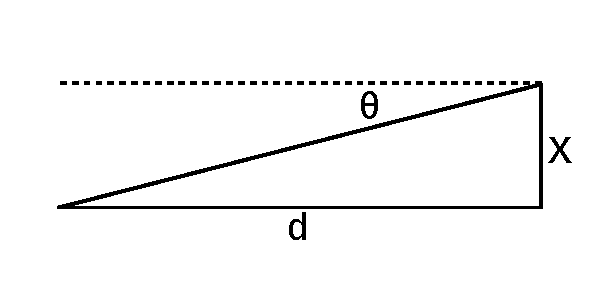
\includegraphics[width=0.49\textwidth]{CompassTriangle.pdf}
\caption{\label{fig:triang} A basic diagram of the triangulation we've performed by walking the baseline $x$ to obtain the distance $d$.}
\end{figure}

\section{Triangulation and Supply Depots}

\begin{enumerate}
\item On the return from the furthest South on the \textit{Discovery} mission, Captain R. F. Scott and his men had marked their supply depots with just one flag.  Why was this dangerous, or what survival asumption tended to be violated in their attempt to find the depots? \\ \vspace{3cm}
\item Suppose you are 10 km away from a supply depot.  At 2 km per hour, in how many hours will you reach the depot? \\ \vspace{2cm}
\item Notice an assumption in the previous exercise is that you are traveling in a straight line.  Suppose the supply depot is at the origin, and you are South of the origin by 10 km.  Draw a 2D coordinate system that depicts your location and the location of the depot. \\ \vspace{4cm}
\item Traveling directly North minimizes the time to locating the depot.  However, suppose you are traveling \textit{5 degrees away from North}.  Where will you arrive in 5 hours, if you are traveling at 2 km per hour? \\ \vspace{3cm}
\item The Norwegian expeditions used a special flagging technique to mark depots.  They placed flags along a \textit{line of longitude} extending to both sides of the depot.  On your figure, mark regular intervals of 0.25 km to either side (horizontally) of your supply depot at the origin.  You get 5 flags on each side, and one at the origin.
\item Suppose when your y-coordinate is zero, you spot a flag.  Calculate the maximum time required to reach the depot.
\end{enumerate}

\end{document}
